\begin{center}
	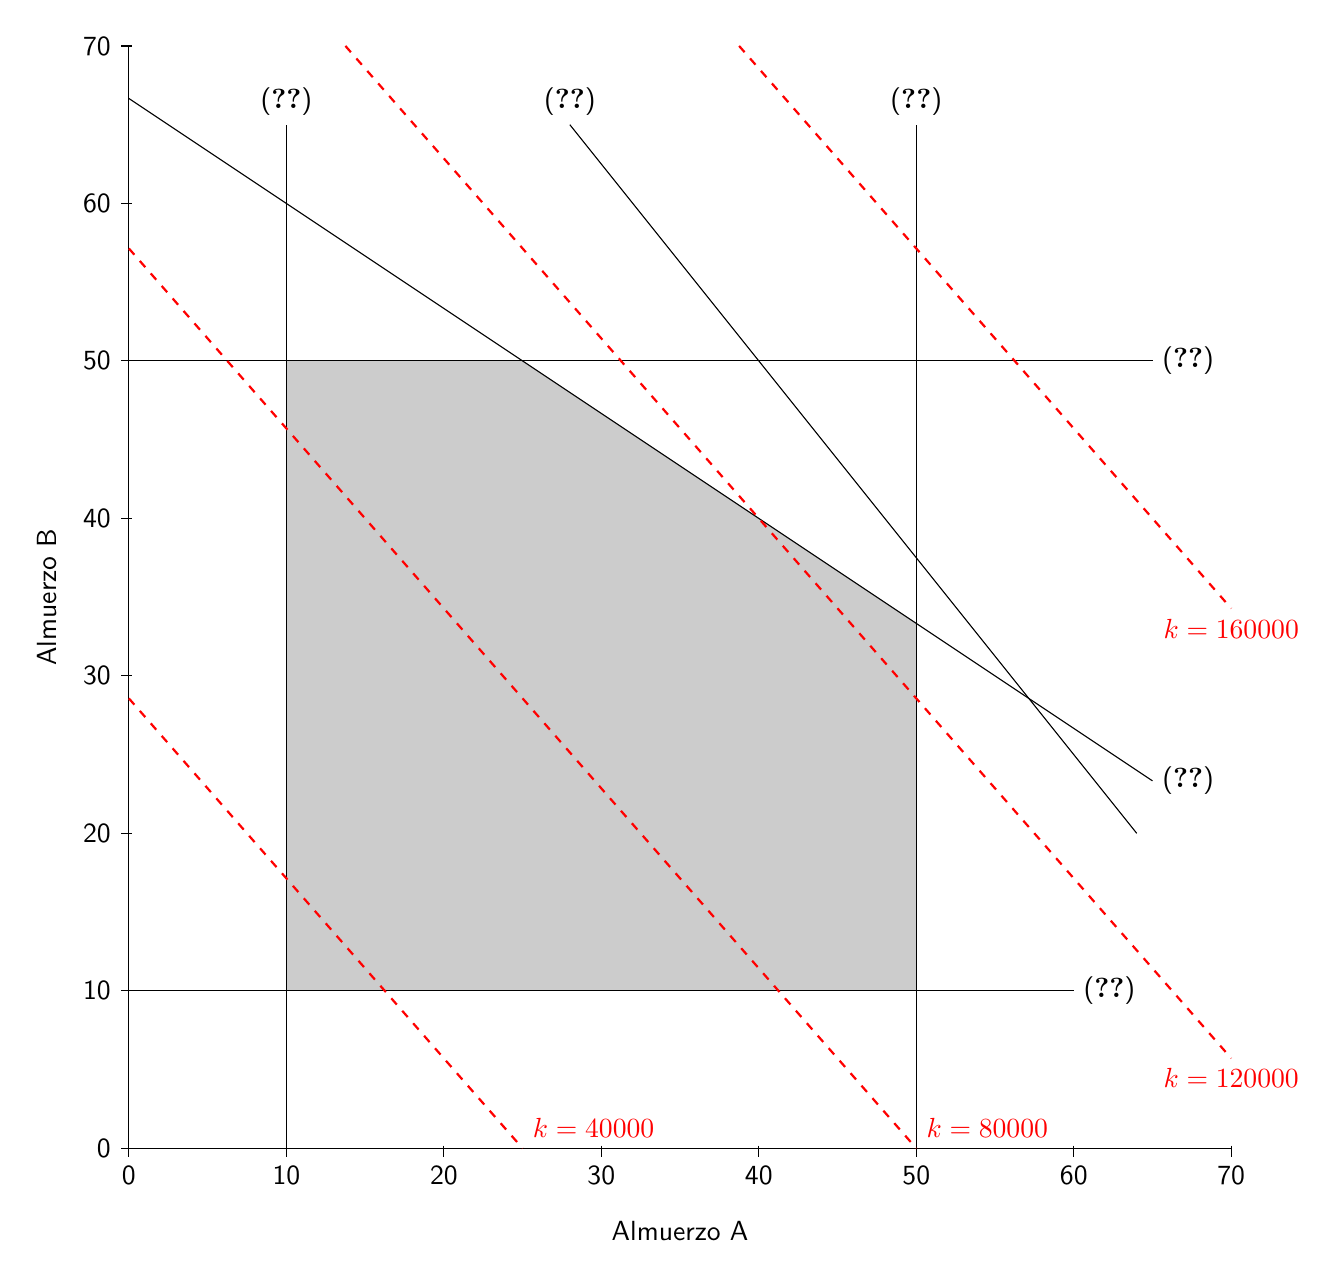
\begin{tikzpicture}[y=.2cm, x=.2cm,font=\sffamily]
		%ejes
		\draw (0,0) -- coordinate (x axis mid) (70,0);
		\draw (0,0) -- coordinate (y axis mid) (0,70);
		%inter
		\foreach \x in {0,10,...,70}
			\draw (\x,1pt) -- (\x,-3pt)
			node[anchor=north] {\x};

		\foreach \y in {0,10,...,70}
			\draw (1pt,\y) -- (-3pt,\y) 
			node[anchor=east] {\y}; 
		%label
		\node[below=0.8cm] at (x axis mid) {Almuerzo A};
		\node[rotate=90, above=0.8cm] at (y axis mid) {Almuerzo B};
		%area
		\fill[gray!40] 
			(10, 10) --
			(10, 50) --
			(25, 50) -- 
			(50, 33.33) --
			(50, 10) -- cycle;
		%lineas
		\draw (10,00) -- (10,65) node[above] {(\ref{1:5})};
		\draw (00,10) -- (60,10) node[right] {(\ref{1:6})};
		\draw (00,50) -- (65,50) node[right] {(\ref{1:4})};
		\draw (50,00) -- (50,65) node[above] {(\ref{1:3})};
		\draw (64,20) -- (28,65) node[above] {(\ref{1:1})};
		\draw (00,66.6666) -- (65,23.3333) node[right] {(\ref{1:2})};
		%f. obj
		\draw[red,thick,dashed]
			(00, 28.57) -- (25, 00) node[above right] {$k=40000$};
		\draw[red,thick,dashed]
			(00, 57.14) -- (50, 00) node[above right] {$k=80000$};
		\draw[red,thick,dashed] 
			(13.75, 70) -- (70, 5.714) node[below] {$k=120000$};
		\draw[red,thick,dashed] 
			(38.75, 70) -- (70, 34.28) node[below] {$k=160000$};
	\end{tikzpicture}
\end{center}
